\chapter*{Update Anaconda dan Spyder}

\begin{enumerate}
	\item Buka anaconda navigator lalu pilih environment
	\begin{figure} [h]
	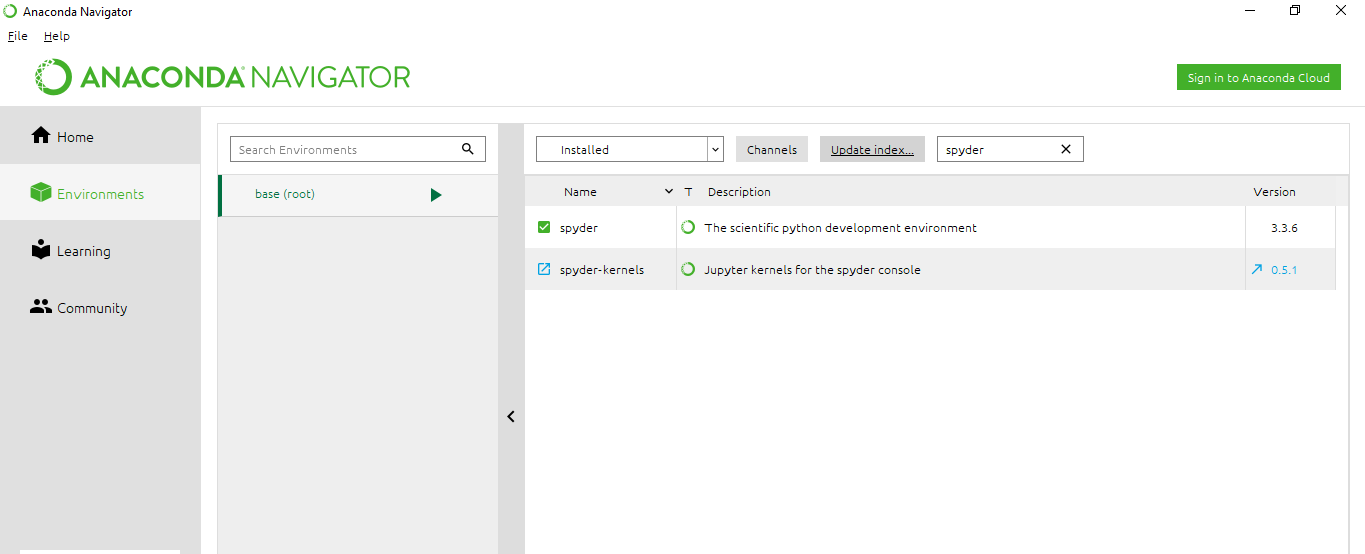
\includegraphics[width=12cm]{section/spy/spy1.png}
	\centering
	\end{figure}
	
    \item untuk update anaconda dan spyder memiliki cara yang sama, hanya berbeda saat di menu search. kalian bsa memilih spyder untuk mengupdate spyder. dan memilih anaconda untuk mengupdate anaconda
	\begin{figure} [h]
	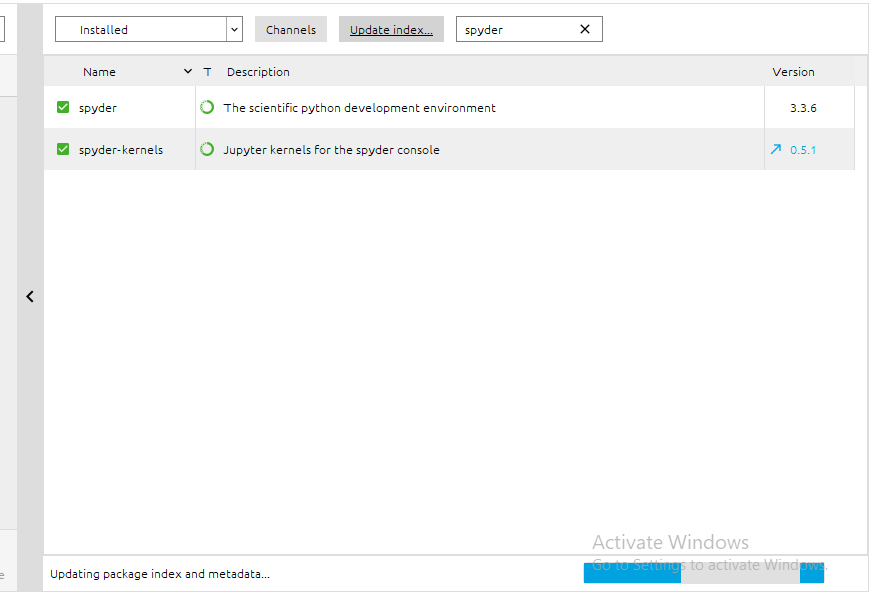
\includegraphics[width=12cm]{section/spy/spy2.png}
	\centering
	\end{figure}
	
	\item klik yang kalian ingin update dan pilih update index
	
	
	\item pilih update index
	\begin{figure} [h]
	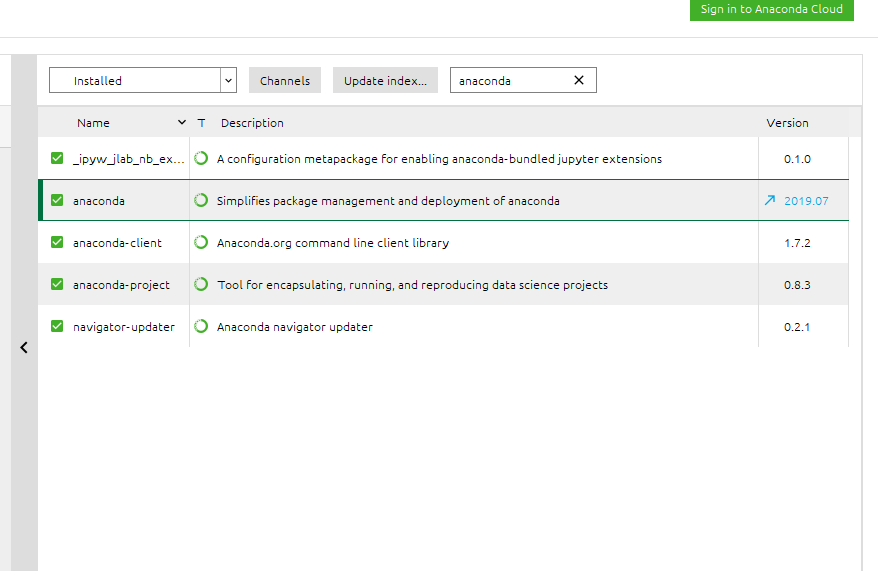
\includegraphics[width=9cm]{section/spy/spy3.png}
	\centering
	\end{figure}
	
	\item maka anaconda atau spyder sudah diupdate
	
	
	
\end{enumerate}